\part{Introduction}

Scania systems are made of a diverse multitude of Electronic Control Units (ECUs) with varying features and constraints, with newer hardware with richer capabilities set to join down the pipeline. Repurposing some of the older hardware and utilising the incoming powerful hardware for machine learning (ML) applications provide an exciting frontier.

\chapter{Background}

Tiny Machine Learning (Tiny ML) is a field of study in embedded systems and machine learning that is growing at a fast pace and has a lot of relevance to this project.

\section{Scania Embedded Systems}

Nature of the Distributed Network

\subsection[Target Hardware]{Target Hardware \linebreak[2]Raspberry Pi Zero}

The Constraints on the Environment

\section{Anomally Detection}

Explain the problem and introduce some terminology which will appear again in the next chapter \dots

\subsubsection{Why perform training and inference on ECUs?}
State the Motivation

\section{Implementations using General Frameworks}

Training and inference of (small) neural networks in embedded systems can be considerably improved compared to general purpose neural networks frameworks

    % \begin{figure}[!ht]
    % 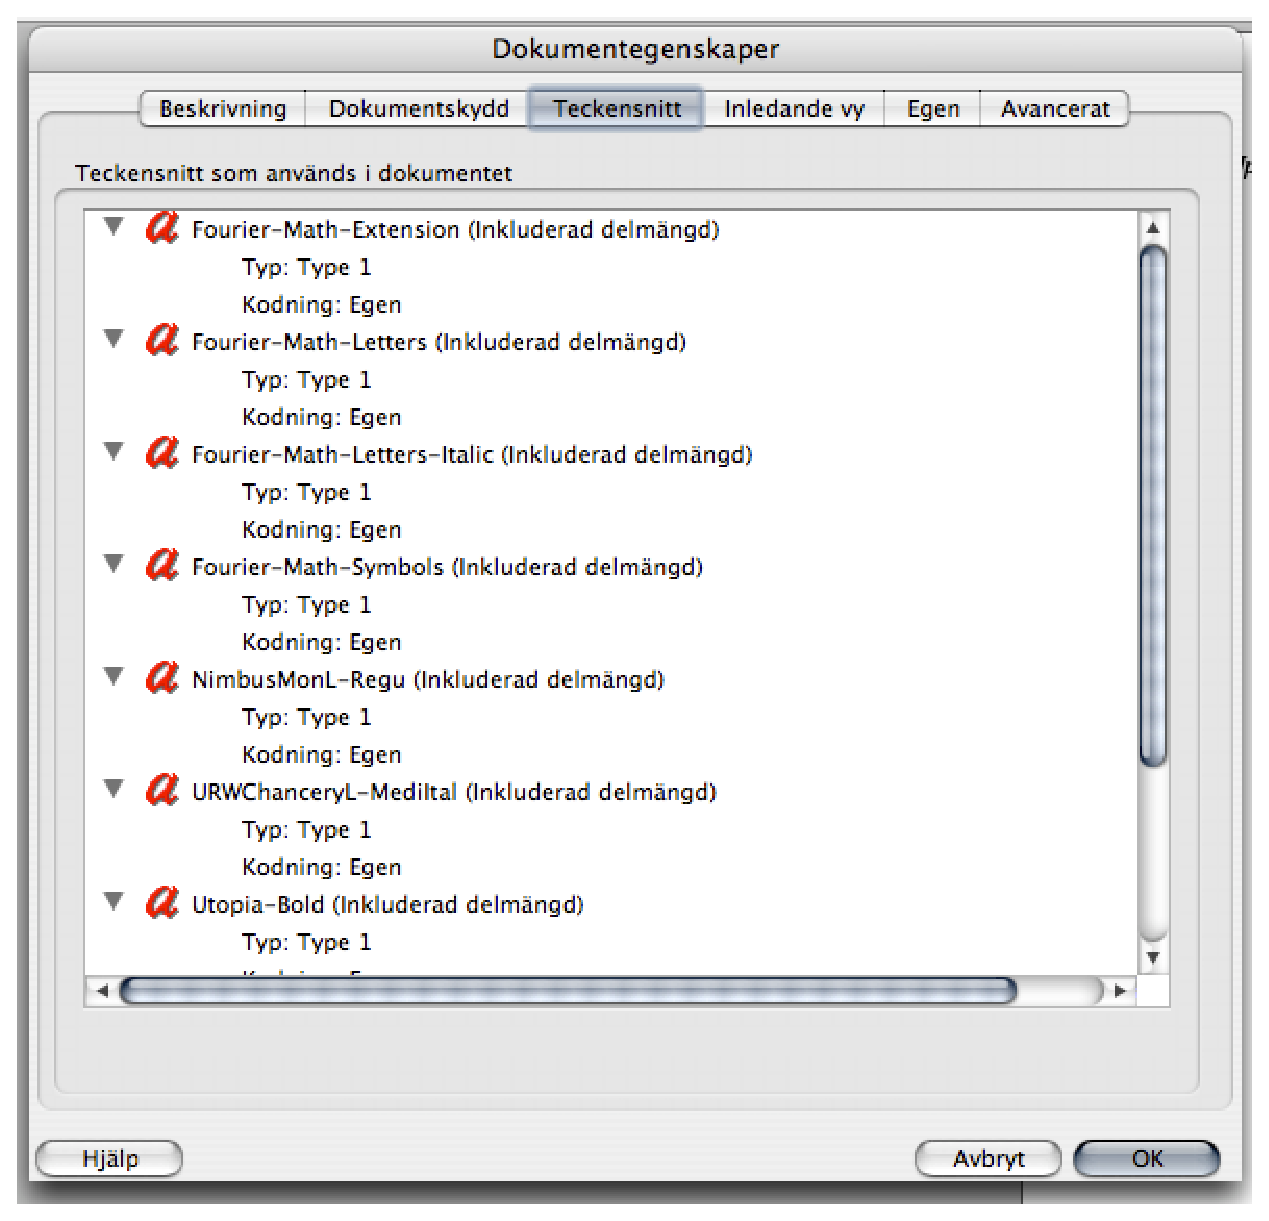
\includegraphics[width=12cm]{Example/Fonts}
	% \caption{Acrobat document properties and fonts display}
    % \end{figure}

% \vspace{\baselineskip}
% \noindent Please send any questions, comments or macro contributions to\\espik@ub.uu.se.

\chapter{Theory}
This section will elaborate and build upon all the theoretical foundations required to implement most of the methods presented in this report.

\section{Pruning}

\section{Quantisation}